%%%%%%%%%%%%%%%%%%%%%%%%%%%%%%%%%%%%%%%%%%%%%%%%%%%%%%%%%%%%%%%%%%%%%%%%%%%%%%%%%%%%
% Document data
%%%%%%%%%%%%%%%%%%%%%%%%%%%%%%%%%%%%%%%%%%%%%%%%%%%%%%%%%%%%%%%%%%%%%%%%%%%%%%%%%%%%
\documentclass[12pt]{article} %report allows for chapters
%%%%%%%%%%%%%%%%%%%%%%%%%%%%%%%%%%%%%%%%%%%%%%%%%%%%%%%%%%%%%%%%%%%%%%%%%%%%%%%%%%%%
\usepackage{preamble}

\begin{document}

\begin{center}
   \textsc{\large MATH 271, Homework 5, \emph{Solutions}}\\
   \textsc{Due October 11$^\textrm{th}$}
\end{center}
\vspace{.5cm}

\begin{problem} $p$-series are actually related to a very important function called the \emph{Riemann zeta function}.  This function is involved in a million dollar math problem! If you're interested in other million dollar problems, look up the Clay Institute Millennium Problems. The Riemann zeta function is given by
\[
\zeta (s) = \sum_{n=1}^\infty \frac{1}{n^s}.
\]
\begin{enumerate}[(a)]
    \item Use the integral test to show that the $p$-series
    \[
    \sum_{n=1}^\infty \frac{1}{n^2}
    \]
    converges.  Look up what this series converges to and write it down. This is $\zeta(2)$.
    \item Use the comparison test to show that the $p$-series
    \[
    \sum_{n=1}^\infty \frac{1}{n^3}
    \]
    converges. This converges as well to $\zeta(3)$. Look up what this approximate value is.
\end{enumerate}
\end{problem}
\begin{solution}~
\begin{enumerate}[(a)]
    \item Note that $a_n = f(n)=\frac{1}{n^2}$.  Hence we can make a comparison to the integral
    \[
    \int_1^\infty f(x)dx,
    \]
    where we start at $x=1$ since our sum begins there as well.  We evaluate the integral
    \begin{align*}
        \int_1^\infty f(x)dx &= \int_1^\infty \frac{1}{x^2}dx\\
        &= \left[\frac{-1}{x}\right]_1^\infty\\
        &= \lim_{b\to \infty} \left[ \frac{-1}{x}\right]_1^b\\
        &= \lim_{b\to \infty} \frac{-1}{b} - \frac{-1}{1}\\
        &= 1.
    \end{align*}
    So since the integral is finite the series converges.  \emph{Warning: the integral does \underline{not} tell us what the series converges to! The series in fact converges to $\zeta(2)=\frac{\pi^2}{6}$.}
    \item Note that for $N\geq 2$ we have that $b_n=\frac{1}{n^3}\leq \frac{1}{n^2}=a_n$. Thus, since we have this inequality and we found $\sum_{n=1}^\infty a_n$ converges, we also have that $\sum_{n=1}^\infty b_n$ converges as well. \emph{Warning: again, this comparison test does \underline{not} tell us what the series converges to. If we look it up we find that $\zeta(3)\approx 1.20206$.}
\end{enumerate}
\end{solution}


\newpage
\begin{problem}
Find the radius of convergence for the following power series
\begin{enumerate}[(a)]
    \item $\displaystyle{\sum_{n=1}^\infty \frac{x^n}{n(n+1)}}$;
    \item $\displaystyle{\sum_{n=0}^\infty \frac{x^{2n+1}}{(2n+1)!}}$.
\end{enumerate}
\end{problem}
\begin{solution}~
\begin{enumerate}[(a)]
    \item To find the radius of convergence we must look at the ratio of terms in the sequence as $n\to \infty$. Specifically, we take
    \begin{align*}
        \lim_{n\to \infty} \left| \frac{\frac{x^{n+1}}{(n+1)(n+2)}}{\frac{x^n}{n(n+1)}}\right| &= \lim_{n\to \infty}\left| \frac{nx}{n+2}\right|\\
        &= |x|.
    \end{align*}
    Now, in order for this series to converge, the ratio test above must give us a limit $L<1$, and hence we must have that $|x|<1$. So the radius of convergence is 1.
    \item Similarly, we have
    \begin{align*}
        \lim_{n\to \infty} \left| \frac{\frac{x^{2n+3}}{(2n+3)!}}{\frac{x^{2n+1}}{(2n+1)!}} \right| &= \lim_{n\to \infty} \left|\frac{x^2}{(2n+3)(2n+2)}\right|\\
        &= 0.
    \end{align*}
    Hence the limit is $0<1$ and so for any value of $x$ this series converges and it follows that the radius of convergence is infinite.
\end{enumerate}
\end{solution}

\newpage
\begin{problem}
Consider the two series
\[
\cos(x) = \sum_{n=0}^\infty \frac{(-1)^n x^{2n}}{(2n)!} \qquad \textrm{and} \qquad \sin(x) = \sum_{n=0}^\infty \frac{(-1)^n x^{2n+1}}{(2n+1)!}.
\]
\begin{enumerate}[(a)]
    \item Show that $\cos(-x)=\cos(x)$.
    \item Show that $\sin(-x)=-\sin(x)$.
    \item To take a derivative of a power series $f(x) = \displaystyle{\sum_{n=0}^\infty a_n x^n}$ we can do the following: 
    \[
    \frac{d}{dx}f(x) = \frac{d}{dx} \sum_{n=0}^\infty a_n x^n = \sum_{n=0}^\infty a_n \frac{d}{dx} x^n.
    \]
    Compute $\frac{d}{dx} \sin(x)$ and $\frac{d}{dx} \cos(x)$ and show that they are equal to what you already know. \emph{Warning: be careful with the powers of $x$ in the case with $\sin$ and $\cos$!}
\end{enumerate}
\end{problem}
\begin{solution}~
\begin{enumerate}[(a)]
    \item We take
    \begin{align*}
        \cos(-x)=\sum_{n=0}^\infty \frac{(-1)^n (-x)^{2n}}{(2n)!} &= \sum_{n=0}^\infty \frac{(-1)^n \left((-x)^2\right)^n}{(2n)!}\\
        &= \sum_{n=0}^\infty \frac{(-1)^n x^{2n}}{(2n)!}\\
        &= \cos(x).
    \end{align*}
    Fundamentally, this is because all powers of $x$ in the terms in the series are even.  This is why we call $\cos$ an \emph{even} function!
    \item Similarly, we take
    \begin{align*}
        \sin(-x)=\sum_{n=0}^\infty \frac{(-1)^n (-x)^{2n+1}}{(2n+1)!}&= \sum_{n=0}^\infty \frac{(-1)^n (-x)\cdot (-x)^{2n}}{(2n+1)!}\\
        &= -\sum_{n=0}^\infty \frac{(-1)^n x\cdot x^{2n}}{(2n+1)!}\\
        &= -\sum_{n=0}^\infty \frac{(-1) x^{2n+1}}{(2n+1)!}\\
        &= -\sin(x).
    \end{align*}
    Again, this is happening due to the fact that all powers of $x$ in the terms for the series are odd. This is why we call $\sin$ an \emph{odd} function.
    \item Consider first $\frac{d}{dx} \sin(x)$.  We take
    \begin{align*}
        \frac{d}{dx} \sum_{n=0}^\infty \frac{(-1)^n x^{2n+1}}{(2n+1)!} &= \frac{d}{dx} \left( x-\frac{x^3}{3!}+\frac{x^5}{5!} - \cdots \right)\\
        &= \frac{d}{dx} x -\frac{d}{dx} \frac{x^3}{3!} +\frac{d}{dx} \frac{x^5}{5!} - \cdots\\
        &= 1 - \frac{x^2}{2!} +\frac{x^4}{4!} - \cdots.
    \end{align*}
    These are the first few terms of the $\cos(x)$ series.  Notice if we take
    \[
    \frac{d}{dx} \frac{(-1)^n x^{2n+1}}{(2n+1)!} = \frac{(-1) x^{2n}}{(2n)!}.
    \]
    So we have
    \[
    \frac{d}{dx} \sin(x) = \cos(x).
    \]
    
    When we consider $\frac{d}{dx}$ of $\cos(x)$ we have to be a bit more careful.  Let's see what happens.  We take
    \begin{align*}
        \frac{d}{dx} \sum_{n=0}^\infty \frac{(-1)^n x^{2n}}{(2n)!} &= \frac{d}{dx} \left(1-\frac{x^2}{2!}+\frac{x^4}{4!} - \cdots \right)\\
        &= \frac{d}{dx} 1 -\frac{d}{dx} \frac{x^2}{2!} +\frac{d}{dx} \frac{x^4}{4!} - \cdots\\
        &= 0 - x +\frac{x^3}{3!} - \cdots
    \end{align*}
    which look like the first terms in the series for $-\sin(x)$. However, let's take a derivative of the term
    \[
    \frac{d}{dx} \frac{(-1)^n x^{2n}}{(2n)!} = \frac{(-1)^n x^{2n-1}}{(2n-1)!}.
    \]
    Now if we were to have this in our series we find
    \[
        \frac{d}{dx} \sum_{n=0}^\infty \frac{(-1)^n x^{2n}}{(2n)!} \not=  \sum_{n=0}^\infty \frac{(-1)^n x^{2n-1}}{(2n-1)!},
    \]
    since the first term on the right has an $x^{-1}$ in it! When we write out the terms of the series and differentiate them, we don't make this mistake.  We just have to be careful.  What we really should have is
    \begin{align*}
                \frac{d}{dx} \sum_{n=0}^\infty \frac{(-1)^n x^{2n}}{(2n)!} &=  \sum_{n=1}^\infty \frac{(-1)^n x^{2n-1}}{(2n-1)!}\\
                &=\sum_{n=0}^\infty \frac{(-1)^{n+1} x^{2n+1}}{(2n+1)!}\\
                &= -\sin(x).
    \end{align*}
    Notice above I \emph{reindexed} the series.  This is not something I'm going to worry too much about you doing.
\end{enumerate}
\end{solution}
\begin{remark}
Again, some of my work here is beyond what I was expecting. If you would have taken the derivatives of the first few terms and showed they are equal, you can extrapolate beyond that and assume it will work for the rest of the terms.  Just be careful with this!
\end{remark}


\newpage
\begin{problem} Consider the function
\[
f(x)=\frac{1}{1-x}.
\]
\begin{enumerate}[(a)]
    \item Compute the Maclaurin series for the function.
    \item Find the integral $\int \frac{dx}{1-x}$ using the Maclaurin series for $f(x)$ found in (a).  
    \item Write down the Maclaurin series for $\ln(1-x)$ and compare to your answer in (b).
\end{enumerate}
\end{problem}
\begin{solution}~
\begin{enumerate}[(a)]
    \item To find the Maclaurin series (i.e., the Taylor series centered at $a=0$), we must compute $f^{(n)}(0)$ as we desire to find
    \[
    f(x) = \sum_{n=0}^\infty \frac{f^{(n)}(0)}{n!}x^n.
    \]
    The derivatives are
    \begin{align*}
        f^{(0)}(x) &= \frac{1}{1-x} &\implies&& f^{(0)}(0)&=1=0!\\
        f^{(1)}(x) &= \frac{1}{(1-x)^2} &\implies&& f^{(1)}(0)&=1=1!\\
        f^{(2)}(x) &= \frac{2}{(1-x)^3} &\implies&& f^{(2)}(0)&=2=2!\\
        f^{(3)}(x) &= \frac{6}{(1-x)^4} &\implies&& f^{(3)}(0)&=6=3!\\
        f^{(4)}(x) &= \frac{24}{(1-x)^5} &\implies&& f^{(4)}(0)&=24=4!\\
        && \vdots && &\\
        f^{(n)}(x) &= \frac{n!}{(1-x)^{n+1}} &\implies&& f^{(n)}(0)&=n!.\\
    \end{align*}
    Hence, if we plug this into the formula for the Maclaurin series we have
    \[
    f(x) = \sum_{n=0}^\infty x^n.
    \]
    \item We can integrate this series term by term to find the desired antiderivative. So we have
    \[
    \int\frac{dx}{1-x} = \int \sum_{n=0}^\infty x^n dx = C + \sum_{n=0}^\infty \frac{x^{n+1}}{n+1}.
    \]
    \item We can find the Maclaurin series for $\ln(1-x)$ in the same way as above. However, notice that $\frac{d}{dx} \ln(1-x) =\frac{-1}{1-x}$, and thus up to determining the constant $C$, we have that
    \[
    -\left(C + \sum_{n=0}^\infty \frac{x^{n+1}}{n+1}\right) = \ln(1-x).
    \]
\end{enumerate}
\end{solution}

\newpage
\begin{problem}~
\begin{enumerate}[(a)]
    \item Compute the Taylor series centered at $a=0$ for $f(x)=e^{-\frac{x^2}{2}}$.
    \item Use the Taylor series for $e^x$ and modify it to find a power series for $f(x)$. Is this the same as the series in (a)?
    \item Plot the original function $f(x)$ compared to the first, second, third, and fourth term approximation for the series on the same graph.
\end{enumerate}
\end{problem}
\begin{solution}
\begin{enumerate}[(a)]
    \item We find the Taylor series centered at $a=0$ by computing $f^{(n)}(0)$. The derivatives are
    \begin{align*}
        f^{(0)}(x) &= e^{-\frac{x^2}{2}} &\implies&& f^{(0)}(0)&=1\\
        f^{(1)}(x) &= xe^{-\frac{x^2}{2}} &\implies&& f^{(1)}(0)&=0\\
        f^{(2)}(x) &= (x^2-1)e^{-\frac{x^2}{2}} &\implies&& f^{(2)}(0)&=-1\\
        f^{(3)}(x) &= x(x^2-3)e^{-\frac{x^2}{2}} &\implies&& f^{(3)}(0)&=0\\
        f^{(4)}(x) &= (x^4-6x^2+3)e^{-\frac{x^2}{2}} &\implies&& f^{(4)}(0)&=3.
    \end{align*}
    This gives us the first five terms of the Taylor series for $f(x)$ so that we have
    \[
    f(x)\approx 1 + 0 + \frac{-1}{2}x^2 + 0 + \frac{3}{4!}x^4.
    \]
    
    \item The easier way is to modify an already known power series like $e^x$. We have
    \[
    e^x = \sum_{n=0}^\infty \frac{x^n}{n!}.
    \]
    If we replace $x\mapsto -\frac{x^2}{2}$ then we have
    \[
    e^{-\frac{x^2}{2}} = \sum_{n=0}^\infty \frac{ \left( -\frac{x^2}{2}\right)}{n!} = \sum_{n=0}^\infty \frac{(-1)^n x^{2n}}{2^n n!}.
    \]
    
    \item Below is a graph showing the three different functions.
    \begin{figure}[H]
        \centering
        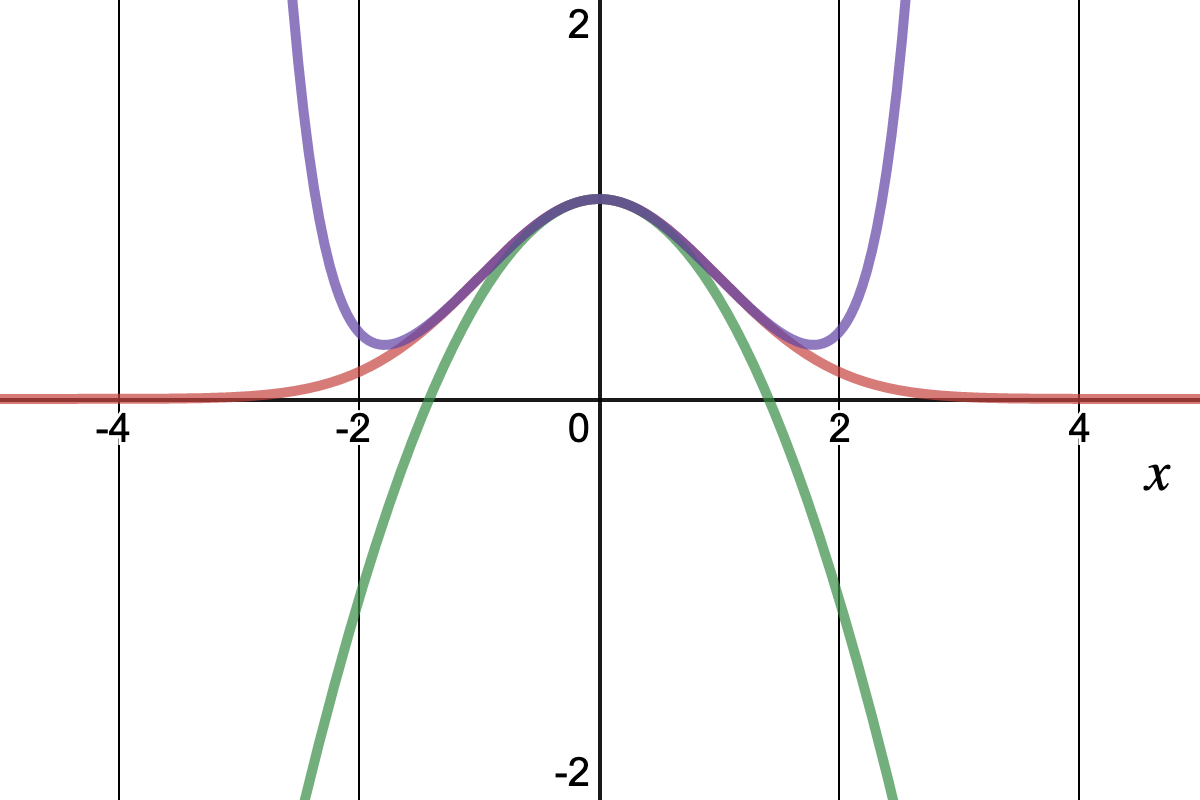
\includegraphics[width=.8\textwidth]{desmos-graph(4).png}
        \caption{Red: $f(x)$; Green: Four terms from Taylor series; Purple: Four terms from modified Taylor series.}
        \label{fig:my_label}
    \end{figure}
    \begin{remark}
    The reason why the graphs are different is because the modified series skips the zero terms that show up in the Taylor series computation. So when we plot four terms in the modified series, it is equal to plotting the first eight terms of the actual Taylor series.
    \end{remark}
\end{enumerate}
\end{solution}

\newpage
\begin{problem}
How can we approximate a (possibly complicated) function by using a power series? Why is this useful (specifically for computation on a computer)?
\end{problem}
\begin{solution}
We can often times approximate a function about a point $x=a$ using a truncated Taylor series centered about $a$. What I mean is that we will have a function $f(x)$ which (inside its interval of convergence) will be equal to
\[
f(x)=\sum_{n=0}^\infty \frac{f^{(n)}(a)}{n!}(x-a)^n
\]
This proves to be very useful as we can take finite truncations of the complete power series above. Specifically, we have that
\[
f(x)\approx \sum_{n=0}^N \frac{f^{(n)}(a)}{n!}(x-a)^n.
\]
It turns out that this is a reasonable approximation for $f$ as long as we don't look too far away from $x=a$.  Also, computers really only have the ability to add.  Of course, multiplication is sequential adding, division can be done through subtraction and multiplication, and powers come from sequential multiplication.  The point is, computers work with polynomials (or rational functions) and this gives us a way to realize a complicated non-polynomial function as (approximately) a polynomial function.
\end{solution}


\end{document}